\chapter{База данных Google Fusion Tables, она же ДинамиТ}
\label{ch:dynamite}


\newthought{По-английски эта база данных} в App Inventor называется ``FusiontablesControl'', 
в книге Камриани и Роя\cite{KamrianiAndRoy2016} её называют ``Google Fusion Tables''. 
В русском интерфейсе среды App Inventor эта база называется предлинно: 
<<УправлениеДинамическимиТаблицами>>, а мы эту базу данных назовём кратко <<ДинамиТ>>, 
где заглавная буква Т указывает на <<\textbf{Т}аблицы>>.

Программы, работающие с ДинамиТом, должны получить разрешение у сервера Гугл, то есть должны указать логин и пароль. Есть два варианта:
\begin{itemize}
    \item Разработчик приложения получает API Key и использует его в программе. 
        Но пользователю программы тогда тоже нужно залогиниться для доступа к ДинамиТу. 
    \item Использовать Service Account. Тогда нужно создать 
        файл с логином и паролем (это наш секретный ключик) и получить 
        мейл ``Service Account Email Address'' из Google APIs Console. 
        Затем сообщаем ДинамиТу мейл ``Service Account Email Address'' 
        и загружаем файл с секретным ключиком в своё приложение, 
        и связываем свойство KeyFile с этим файлом. 
        Наконец, в Дизайнере ставим галочку на пункт ``UseServiceAuthentication''. 
        В случае использования Service Account 
        пользователям не нужно заботиться о логине в ДинамиТ, 
        все эти заботы берёт на себя приложение.
\end{itemize}




\section{Приготовление ДинамиТа}


Откройте веб-страницу Google Диска (https://drive.google.com).\marginnote[-0cm]{
    Чтобы получить доступ к Google Диску, достаточно зарегистрироваться на сайте Google.
}
Нажмите последовательно 
кнопки меню: <<Создать>>, <<Ещё>> и~кнопку <<+ Подключить другие приложения>> 
(рис.~\ref{fig:google_drive_connect_more_apps}). В новом окне будет множество 
приложений, которые можно подключить к~Google Диску. 

\begin{figure}
{%
\setlength{\fboxsep}{0pt}%
\setlength{\fboxrule}{1pt}%
\fcolorbox{gray}{gray}{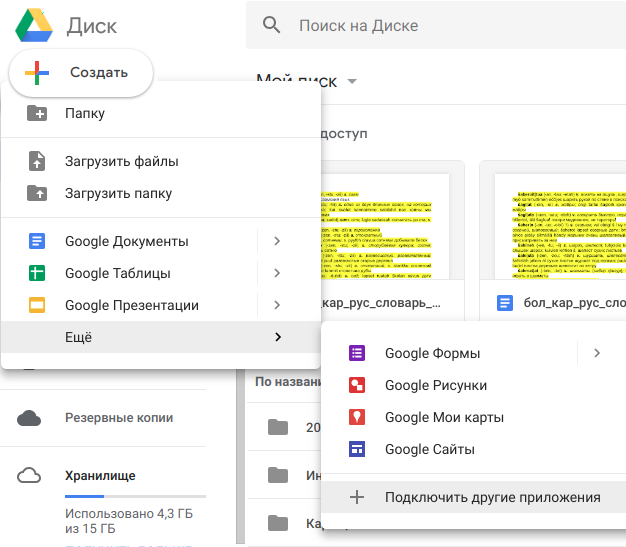
\includegraphics{./lessons/db_google_fusion/020_google_drive_connect_more_apps_with_new-button_ru.png}}%
}%
    \caption[Подключения приложения к Google Диску.][56pt]{Подключения 
            приложения к Google Диску.
    }
  \label{fig:google_drive_connect_more_apps}
\end{figure}

В строке поиска нового окна наберите слово ``Fusion''. Нажмите кнопку поиска. 
Из списка приложений выберите ``Fusion Tables'' и нажмите кнопку <<Подключить>> 
(рис.~\ref{fig:add_fusion_to_drive}).

\begin{figure}
{%
\setlength{\fboxsep}{0pt}%
\setlength{\fboxrule}{1pt}%
\fcolorbox{gray}{gray}{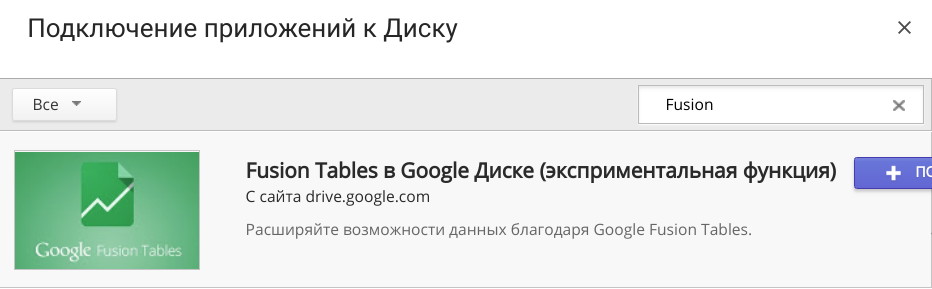
\includegraphics{./lessons/db_google_fusion/030_add_fusion_to_drive_ru.png}}%
}%
    \caption[Выбор приложения в Google Диск.][-0pt]{Выбор приложения 
            ``Fusion Tables'' в Google Диск. У кнопки <<Подключить>> 
            на экране поместились первые полторы буквы.

        { Если даже у Гугля на картинке есть опечатки, то какой может быть 
        спрос с авторов этой книги $\ddot\smile$
        }
    }
  \label{fig:add_fusion_to_drive}
\end{figure}

Теперь, если ещё раз нажать кнопки <<Создать>> и <<Ещё>>, в~списке меню будут 
<<Google Сводные таблицы>> (рис.~\ref{fig:fusion_is_available_at_drive}).

\begin{figure}
{%
\setlength{\fboxsep}{0pt}%
\setlength{\fboxrule}{1pt}%
\fcolorbox{gray}{gray}{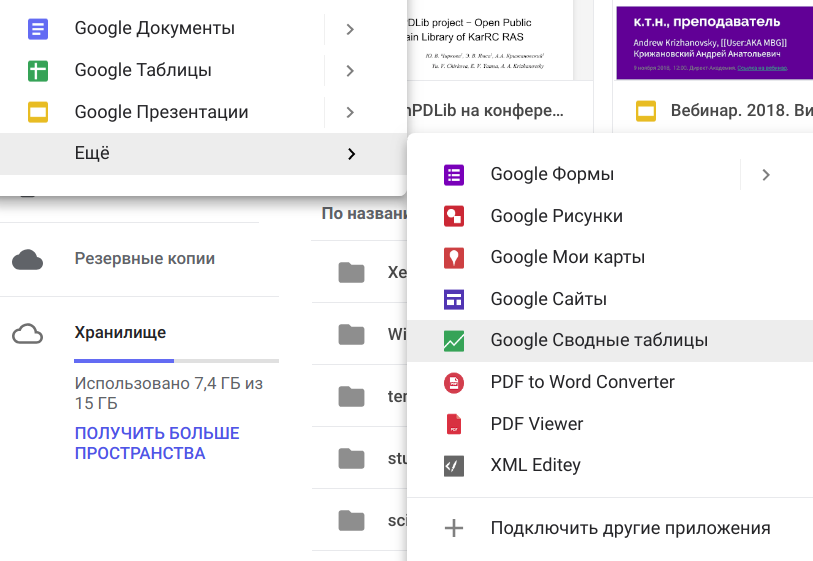
\includegraphics{./lessons/db_google_fusion/040_GoogleFusionTables_avail_ru.png}}%
}%
    \caption[Google Сводные таблицы доступны в Google Диск.][56pt]{Google Сводные таблицы 
            (по-нашему ДинамиТ) доступны в Google Диск.
    }
  \label{fig:fusion_is_available_at_drive}
\end{figure}

Щёлкнем по кнопке <<Google Сводные таблицы>>, чтобы создать новую таблицу.

Откроется новое окно (рис.~\ref{fig:fusion_create_empty_table}). Выберите пункт 
``Create empty table'' для создания новой пустой таблицы.

\begin{figure}
{%
\setlength{\fboxsep}{0pt}%
\setlength{\fboxrule}{1pt}%
\fcolorbox{gray}{gray}{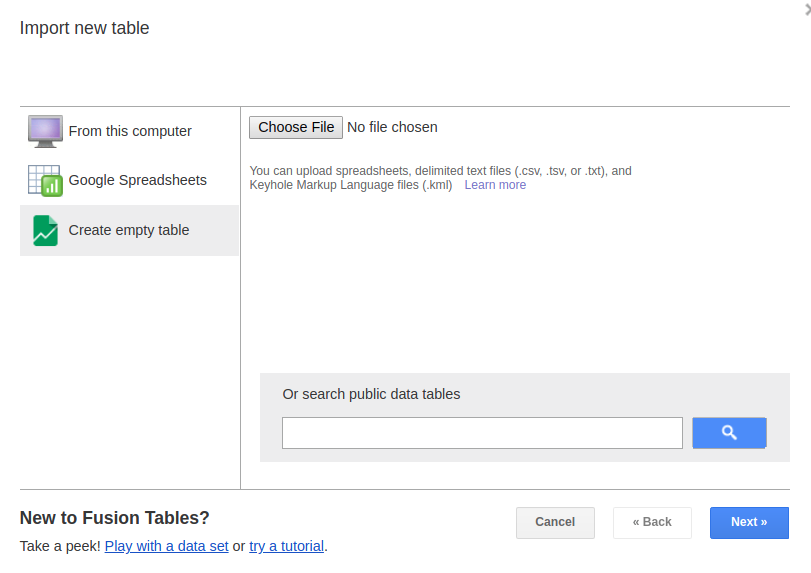
\includegraphics{./lessons/db_google_fusion/050_create_empty_table.png}}%
}%
    \caption[Создание новой Google Сводной таблицы.][0pt]{Создание новой 
            Google Сводной таблицы (Fusion Table).

            { 
                Интерфейс Fusion Tables на русский пока не переведён, 
                но для нас это не беда. 
            }

            {
                Обратите внимание, что внизу иллюстрации есть ссылка на учебник 
                по Fusion Tables: \url{https://support.google.com/fusiontables}.
            }
    }
  \label{fig:fusion_create_empty_table}
\end{figure}


\section{Закладка (данных) ДинамиТа}

Ну вот, наконец, мы добрались до табличной формы, где можно вводить данные в ДинамиТ или Google Сводные таблицы.

Первым делом дадим таблице название и описание (см. рис. 060\_table\_name.png). 
Таблица будет называться ``FlagColor Table''. Затем нажмите кнопку ``Save'', чтобы сохранить название.

\newthought{О пустоте}. Нужна ещё пара штрихов, прежде чем мы сможем использовать эту таблицу в нашем приложении. 
Изначально при создании таблицы в неё вставляется одна пустая строка, а нам нужна совершенно пустая таблицу. Как очистить таблицу? 
Для этого выберите пункт меню ``Edit'', затем ``Delete all rows'' (см. рис. 070\_Edit\_delete\_all\_rows\_to\_clear\_table.png). 
На вопрос -- уверены ли вы, что нужно всё удалить? -- ответьте утвердительно (см. рис. 080\_yes\_delete\_all\_rows.png).


